% !TEX root =  ./main.tex

\section{Toy Example}\label{sec:student}

To illustrate some basic concepts of RSs and, in the next section, of the proposed encoding, we model a system composed of a student and a vending machine as a toy example.
The vending machine accept two different kinds of coins and can dispense either a cappuccino or an expresso when a coffe coin is inserted or a tea if a tea coin is inserted. A cappuccino is dispensed if some milk is available, otherwise the expresso is produced.
Assuming the powder for preparing coffee and tea are always present, the corresponding process can be written as follows:
\[
\begin{array}{lll}
\mathsf{VM} & \triangleq & (\{\ccoin,\cpowder\},\{\nomilk\},\{\cappuccino\})\\
& | & (\{\ccoin,\cpowder,\nomilk\},\emptyset,\{\espresso\})\\
& | & (\{\tcoin,\tpowder\},\emptyset,\{\tea\})\\
& | & (\{\cpowder\},\emptyset,\{\cpowder\})\\
& | & (\{\tpowder\},\emptyset,\{\tpowder\})\\
\end{array}
\]

A refill context process can, nondeterministically, refill the machine with milk.
\[
\begin{array}{lll}
\mathsf{Refill} & \triangleq & \{\nomilk\}.\mathsf{Refill}\\
& + & \emptyset.\mathsf{Refill}\\
\end{array}
\]

The student process is very simple: she takes cappuccino in the morning and tea in the afternoon, otherwise she gets angry.
\[
\begin{array}{rll}
\mathsf{Student} & \triangleq & (\emptyset,\{\am\},\{\tcoin\}).\mathsf{GetTea}\\
& + & (\{\am\},\emptyset,\{\ccoin\}).\mathsf{GetCappuccino}\\
& + & \{\idle\}.\mathsf{Student}\\
\mathsf{GetCappuccino} & \triangleq & (\{\cappuccino\},\emptyset,\emptyset).\mathsf{Student}\\
& + & (\{\espresso\},\emptyset,\{\anger\}).\mathsf{Student}\\
\mathsf{GetTea} & \triangleq & (\{\tea\},\emptyset,\emptyset).\mathsf{Student}\\
& + & (\emptyset,\{\tea\},\{\anger\}).\mathsf{Student}\\
\end{array}
\]

Finally, two more reactions model the passage of time (morning vs afternoon) while the student is idle.
\[
\begin{array}{lll}
\mathsf{Day} & \triangleq & (\{\idle\},\{\am\},\{\am\})\\
& | & (\{\am\},\{\idle\},\textcolor{red}{\{\am\}})
\end{array}
\]

We assume that, initially, both entitites $\cpowder$ and $\tpowder$ are present.
So the system can be written as:
\[
[\,\{\cpowder,\tpowder\} 
| \mathsf{VM}
| \mathsf{Refill}
| \mathsf{Day}
| \mathsf{Student}
\,]
\]

Using BioReSolve, we can generate the underlying LTS as in Fig.~\ref{fig:toylts}: the initial state is in light blue, while the state where the student is angry is in light coral.

\begin{figure}
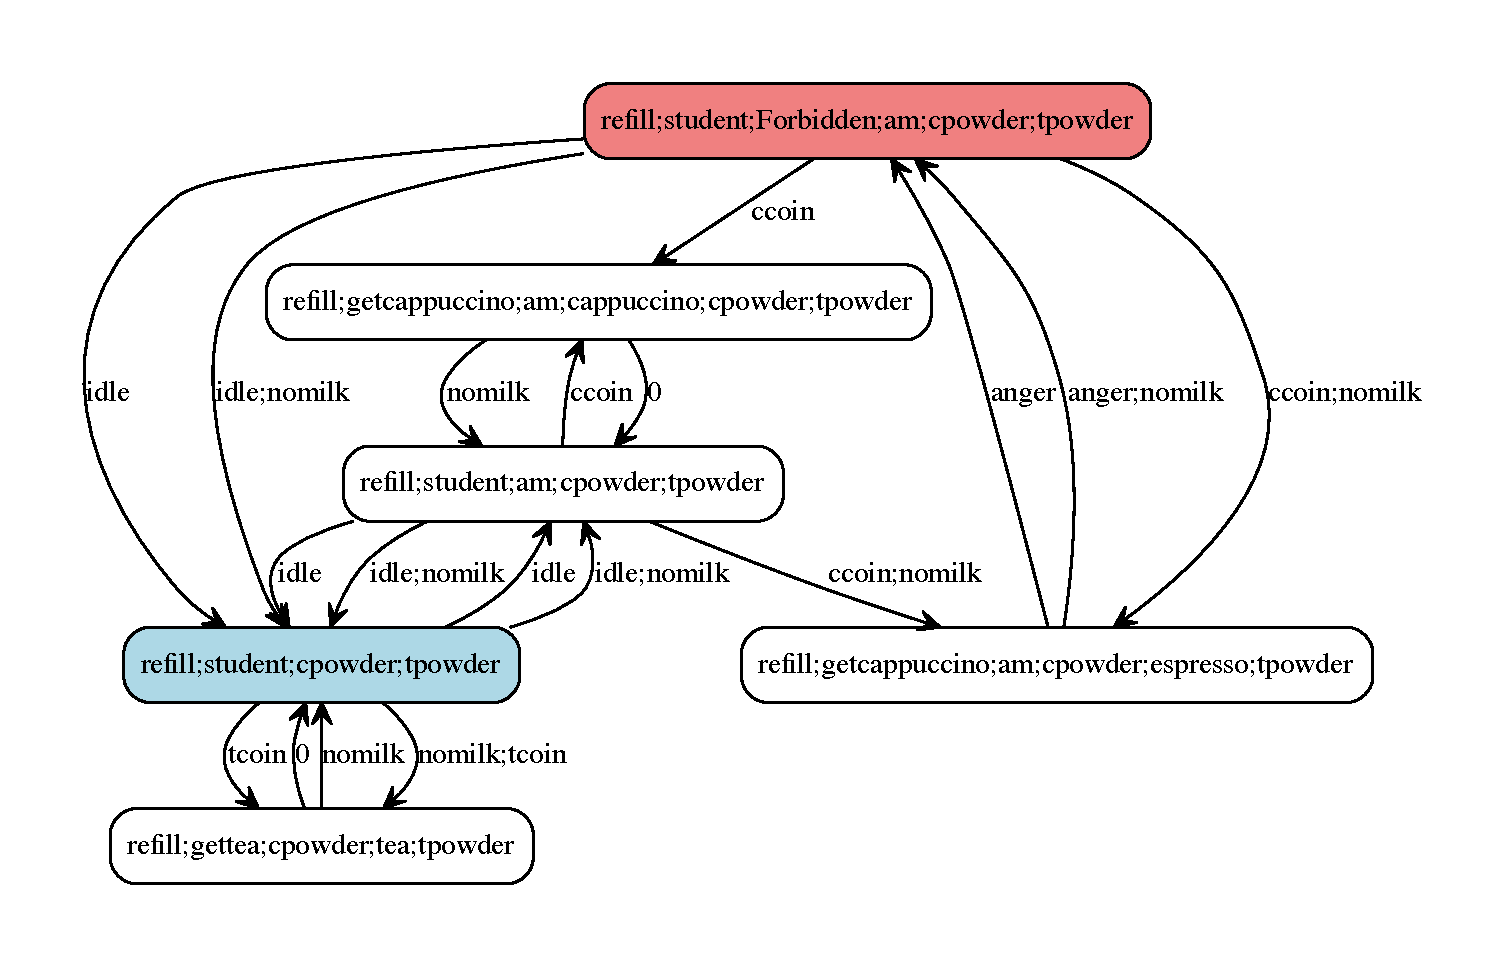
\includegraphics[scale=.3]{toylts}
\caption{LTS of the toy example.}\label{fig:toylts}
\end{figure}